% answers.tex —— 2005 年·上海卷·理科 · 参考答案与详细解析片段
% 由 tools/generate_projects.py 依来源总账自 2005/2005_数学真题_上海理_试题.md + 2005/2005_数学真题_上海理_解析正文.md + 2005/2005_数学真题_上海理_答案要点.md 生成，勿手改（改源 MD 后重跑）


\begin{gktip}
固定候选 PDF 仅含题面，没有答案、解析或评分标准。以下为依据已复核题面独立推导的非官方解析。来源发布者、出版者、版次、复制链和官方身份未核；项目尚未认证官方答案。Q11 的并列最小端点及 Q20(1) 原文“中低价层”均保留 U/PENDING。
\end{gktip}

\begin{answer}
\gksolhead{1}{}

\textbf{题目}：

函数 $f(x)=\log_4(x+1)$ 的反函数 $f^{-1}(x)=\underline{\qquad}$。

\Needspace{4\baselineskip}
\textbf{解析}

\Needspace{5\baselineskip}
由 $y=\log_4(x+1)$ 得 $x=\log_4(y+1)$；因此 $y+1=4^x$，所以

\nopagebreak[4]
\[
f^{-1}(x)=4^x-1\mbox{。}
\]

\gkanswer{答案：$f^{-1}(x)=4^x-1$}

\end{answer}
\begin{answer}
\gksolhead{2}{}

\textbf{题目}：

方程 $4^x+2^x-2=0$ 的解是 $\underline{\qquad}$。

\Needspace{4\baselineskip}
\textbf{解析}

令 $t=2^x>0$，原方程化为 $t^2+t-2=(t+2)(t-1)=0$。由 $t>0$ 得 $t=1$，故 $x=0$。

\gkanswer{答案：$x=0$}

\end{answer}
\begin{answer}
\gksolhead{3}{}

\textbf{题目}：

直角坐标平面 $xOy$ 中，若定点 $A(1,2)$ 与动点 $P(x,y)$ 满足 $\overrightarrow{OP}\cdot\overrightarrow{OA}=4$，则点 $P$ 的轨迹方程是 $\underline{\qquad}$。

\Needspace{4\baselineskip}
\textbf{解析}

\Needspace{5\baselineskip}
由 $\overrightarrow{OP}=(x,y)$、$\overrightarrow{OA}=(1,2)$，点积条件给出

\nopagebreak[4]
\[
x+2y=4\mbox{。}
\]

\gkanswer{答案：$x+2y=4$}

\end{answer}
\begin{answer}
\gksolhead{4}{}

\textbf{题目}：

在 $(x-a)^{10}$ 的展开式中，$x^7$ 的系数是 $15$，则实数 $a=\underline{\qquad}$。

\Needspace{4\baselineskip}
\textbf{解析}

$(x-a)^{10}$ 中 $x^7$ 的系数是 $\binom{10}{3}(-a)^3=-120a^3$。令其等于 $15$，得 $a^3=-\frac18$，所以 $a=-\frac12$。

\gkanswer{答案：$a=-\frac12$}

\end{answer}
\begin{answer}
\gksolhead{5}{}

\textbf{题目}：

若双曲线的渐近线方程为 $y=\pm3x$，它的一个焦点是 $(\sqrt{10},0)$，则双曲线的方程是 $\underline{\qquad}$。

\Needspace{4\baselineskip}
\textbf{解析}

\Needspace{5\baselineskip}
设双曲线为 $\frac{x^2}{a^2}-\frac{y^2}{b^2}=1$。渐近线斜率给出 $\frac ba=3$；焦点坐标给出 $c^2=a^2+b^2=10$。于是 $10a^2=10$，故 $a^2=1$、$b^2=9$，方程为

\nopagebreak[4]
\[
x^2-\frac{y^2}{9}=1\mbox{。}
\]

\gkanswer{答案：$x^2-\frac{y^2}{9}=1$}

\end{answer}
\begin{answer}
\gksolhead{6}{}

\textbf{题目}：

\Needspace{5\baselineskip}
将参数方程

\nopagebreak[4]
\[
\begin{cases}
x=1+2\cos\theta,\\
y=2\sin\theta,
\end{cases}
\]

（$\theta$ 为参数）化为普通方程，所得方程是 $\underline{\qquad}$。

\Needspace{4\baselineskip}
\textbf{解析}

\Needspace{5\baselineskip}
由 $x-1=2\cos\theta$、$y=2\sin\theta$ 及 $\cos^2\theta+\sin^2\theta=1$，得

\nopagebreak[4]
\[
\frac{(x-1)^2}{4}+\frac{y^2}{4}=1\mbox{。}
\]

\gkanswer{答案：$\frac{(x-1)^2}{4}+\frac{y^2}{4}=1$}

\end{answer}
\begin{answer}
\gksolhead{7}{}

\textbf{题目}：

计算：$\displaystyle\lim_{n\to\infty}\frac{3^{n+1}-2^n}{3^n+2^{n-1}}=\underline{\qquad}$。

\Needspace{4\baselineskip}
\textbf{解析}

\Needspace{5\baselineskip}
分子分母同除以 $3^n$：

\nopagebreak[4]
\[
\frac{3-(\frac23)^n}{1+\frac12(\frac23)^n}\longrightarrow 3\mbox{。}
\]

\gkanswer{答案：$3$}

\end{answer}
\begin{answer}
\gksolhead{8}{}

\textbf{题目}：

某班有 $50$ 名学生，其中 $15$ 人选修 $A$ 课程，另外 $35$ 人选修 $B$ 课程。从班级中任选两名学生，他们是选修不同课程的学生的概率是 $\underline{\qquad}$。（结果用分数表示）

\Needspace{4\baselineskip}
\textbf{解析}

\Needspace{5\baselineskip}
两人来自不同课程的选法有 $15\cdot35$ 种，任选两人的总选法为 $\binom{50}{2}$ 种，因此所求概率为

\nopagebreak[4]
\[
\frac{15\cdot35}{\binom{50}{2}}=\frac37\mbox{。}
\]

\gkanswer{答案：$\frac37$}

\end{answer}
\begin{answer}
\gksolhead{9}{}

\textbf{题目}：

在 $\triangle ABC$ 中，若 $A=120^\circ$，$AB=5$，$BC=7$，则 $\triangle ABC$ 的面积 $S=\underline{\qquad}$。

\Needspace{4\baselineskip}
\textbf{解析}

\Needspace{5\baselineskip}
设 $AC=x>0$。由余弦定理，

\nopagebreak[4]
\[
49=25+x^2-2\cdot5x\cos120^\circ=x^2+5x+25\text{，}
\]

\Needspace{5\baselineskip}
所以 $(x+8)(x-3)=0$，从而 $AC=3$。三角形面积为

\nopagebreak[4]
\[
S=\frac12\cdot AB\cdot AC\sin120^\circ=\frac{15\sqrt3}{4}\mbox{。}
\]

\gkanswer{答案：$\frac{15\sqrt3}{4}$}

\end{answer}
\begin{answer}
\gksolhead{10}{}

\textbf{题目}：

函数 $f(x)=\sin x+2|\sin x|$，$x\in[0,2\pi]$ 的图象与直线 $y=k$ 有且仅有两个不同的交点，则 $k$ 的取值范围是 $\underline{\qquad}$。

\Needspace{4\baselineskip}
\textbf{解析}

\Needspace{5\baselineskip}
在 $[0,\pi]$ 上 $\sin x\ge0$，故 $f(x)=3\sin x$；在 $[\pi,2\pi]$ 上 $\sin x\le0$，故 $f(x)=-\sin x$。当 $1<k<3$ 时，水平线 $y=k$ 与前一段恰有两个交点、与后一段无交点。$k=1$ 会在后一段再产生交点，$k=3$ 在前一段只有一个交点；其余 $k$ 也不满足恰有两个不同交点。因此

\nopagebreak[4]
\[
1<k<3\mbox{。}
\]

\gkanswer{答案：$1<k<3$}

\end{answer}
\begin{answer}
\gksolhead{11}{}

\textbf{题目}：

有两个相同的直三棱柱，高为 $\frac{2}{a}$，底面三角形的三边长分别为 $3a,4a,5a$（$a>0$）。用它们拼成一个三棱柱或四棱柱，在所有可能的情形中，全面积最小的是一个四棱柱，则 $a$ 的取值范围是 $\underline{\qquad}$。
\nopagebreak[4]
\begin{center}% Candidate source: src-22a421a422f050bc84accae7bf41feb6903c62df04bd83f34d8267d28f49ee2e
% Source PDF SHA-256: 092e8e90dc1430ab2fa8b8ce79e072e317559e6bef29f1cb7461e9423925ec31
% PDF page 1 (printed page 262), question 11. The two printed sketches are identical.
% Redraw preserves visible/hidden linework; labels do not define drawing scale.
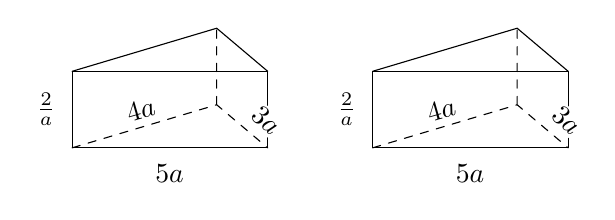
\begin{tikzpicture}[scale=0.72,line cap=round,line join=round]
  \foreach \shift in {0,5.3} {
    \begin{scope}[shift={(\shift,0)}]
      \coordinate (A) at (0,0);
      \coordinate (B) at (3.45,0);
      \coordinate (C) at (2.55,0.76);
      \coordinate (Aone) at (0,1.35);
      \coordinate (Bone) at (3.45,1.35);
      \coordinate (Cone) at (2.55,2.11);

      % Front rectangle and visible upper outline.
      \draw (A)--(B)--(Bone)--(Aone)--cycle;
      \draw (Aone)--(Cone)--(Bone);

      % Hidden base edges and rear vertical edge.
      \draw[dashed] (A)--(C)--(B) (C)--(Cone);

      \node[left] at (-0.12,0.68) {$\frac{2}{a}$};
      \node[below] at (1.72,-0.12) {$5a$};
      \node[above,rotate=16,fill=white,inner sep=1pt] at (1.27,0.46) {$4a$};
      \node[above right,rotate=-42,fill=white,inner sep=1pt] at (3.05,0.53) {$3a$};
    \end{scope}
  }
\end{tikzpicture}
\end{center}
\nopagebreak[4]
\Needspace{4\baselineskip}
\textbf{解析}

\Needspace{5\baselineskip}
三棱柱的底面是边长 $3a,4a,5a$ 的直角三角形，底面积为 $6a^2$、周长为 $12a$。将两个棱柱的三角形端面对接，得到高为 $4/a$ 的三棱柱，其表面积为

\nopagebreak[4]
\[
S_3=2\cdot6a^2+12a\cdot\frac4a=12a^2+48\mbox{。}
\]

\Needspace{5\baselineskip}
沿侧面拼成四棱柱时，共同侧面的宽 $s$ 可为 $3a,4a,5a$。所得底面面积为 $12a^2$，周长为 $24a-2s$，柱高为 $2/a$，故

\nopagebreak[4]
\[
S_4(s)=24a^2+(24a-2s)\frac2a=24a^2+48-\frac{4s}{a}\mbox{。}
\]

四棱柱的表面积在 $s=5a$ 时最小，为 $24a^2+28$。与三棱柱比较，差为 $12a^2-20$。四棱柱严格较小时 $0<a<\sqrt{\frac53}$；$a=\sqrt{\frac53}$ 时二者并列最小。题干未说明“最小的是一个四棱柱”是否允许并列，故端点归属保留 U/PENDING，不选定单一范围。

\gkanswer{答案：U/PENDING}

\end{answer}
\begin{answer}
\gksolhead{12}{}

\textbf{题目}：

\Needspace{5\baselineskip}
用 $n$ 个不同的实数 $a_1,a_2,\cdots,a_n$ 可得到 $n!$ 个不同的排列，每个排列为一行写成一个 $n!$ 行的数阵。对第 $i$ 行 $a_{i1},a_{i2},\cdots,a_{in}$，记

\nopagebreak[4]
\[
b_i=-a_{i1}+2a_{i2}-3a_{i3}+\cdots+(-1)^nna_{in},\qquad i=1,2,3,\cdots,n!.
\]

\Needspace{5\baselineskip}
例如：用 $1,2,3$ 可得数阵如图，由于此数阵中每一列各数之和都是 $12$，所以，

\nopagebreak[4]
\[
b_1+b_2+\cdots+b_6=-12+2\times12-3\times12=-24\text{，}
\]

\Needspace{5\baselineskip}
那么，在用 $1,2,3,4,5$ 形成的数阵中，$b_1+b_2+\cdots+b_{120}=\underline{\qquad}$。

\nopagebreak[4]
\[
\begin{array}{ccc}
1&2&3\\
1&3&2\\
2&1&3\\
2&3&1\\
3&1&2\\
3&2&1
\end{array}
\]

\Needspace{4\baselineskip}
\textbf{解析}

\Needspace{5\baselineskip}
每个数在每一列中均出现 $4!=24$ 次，所以用 $1,2,3,4,5$ 排列时每列之和都是 $24(1+2+3+4+5)=360$。因此

\nopagebreak[4]
\[
\sum_{i=1}^{120}b_i=(-1+2-3+4-5)\cdot360=-1080\mbox{。}
\]

\gkanswer{答案：$-1080$}

\end{answer}
\begin{answer}
\gksolhead{13}{}

\textbf{题目}：

若函数 $f(x)=\dfrac{1}{2^x+1}$，则该函数在 $(-\infty,+\infty)$ 上是\mbox{（　　）}。

（A）单调递减无最小值　　（B）单调递减有最小值

（C）单调递增无最大值　　（D）单调递增有最大值

\Needspace{4\baselineskip}
\textbf{解析}

$2^x+1$ 为正且严格递增，故其倒数 $f(x)=\frac1{2^x+1}$ 严格递减。函数值恒大于 $0$，下确界 $0$ 不取到，所以无最小值，选 A。

\gkanswer{答案：A}

\end{answer}
\begin{answer}
\gksolhead{14}{}

\textbf{题目}：

已知集合 $M=\{x\mid |x-1|\leqslant2,\ x\in\mathbb R\}$，$P=\left\{x\mid\dfrac{5}{x+1}\geqslant1,\ x\in\mathbb Z\right\}$，则 $M\cap P$ 等于\mbox{（　　）}。

（A）$\{x\mid 0<x\leqslant3,\ x\in\mathbb Z\}$　　（B）$\{x\mid 0\leqslant x\leqslant3,\ x\in\mathbb Z\}$

（C）$\{x\mid -1\leqslant x\leqslant0,\ x\in\mathbb Z\}$　　（D）$\{x\mid -1\leqslant x<0,\ x\in\mathbb Z\}$

\Needspace{4\baselineskip}
\textbf{解析}

\Needspace{5\baselineskip}
由 $|x-1|\le2$ 得 $M=[-1,3]$。集合 $P$ 中须有 $x\ne-1$，且

\nopagebreak[4]
\[
\frac{5}{x+1}\ge1\iff\frac{4-x}{x+1}\ge0\iff -1<x\le4\mbox{。}
\]

结合 $x\in\mathbb Z$ 与 $M$，得到 $M\cap P=\{0,1,2,3\}$，选 B。

\gkanswer{答案：B}

\end{answer}
\begin{answer}
\gksolhead{15}{}

\textbf{题目}：

过抛物线 $y^2=4x$ 的焦点作一条直线与抛物线相交于 $A$、$B$ 两点，它们的横坐标之和等于 $5$，则这样的直线\mbox{（　　）}。

（A）有且仅有一条　　（B）有且仅有两条

（C）有无穷多条　　（D）不存在

\Needspace{4\baselineskip}
\textbf{解析}

\Needspace{5\baselineskip}
设过焦点 $(1,0)$ 的非竖直直线为 $y=m(x-1)$。代入 $y^2=4x$，两交点横坐标满足

\nopagebreak[4]
\[
m^2x^2-(2m^2+4)x+m^2=0\text{，}
\]

故其和为 $2+\frac4{m^2}$。令其等于 $5$，得 $m^2=\frac43$，有斜率相反的两条直线，选 B。竖直直线 $x=1$ 的两个交点横坐标之和为 $2$，不符合条件。

\gkanswer{答案：B}

\end{answer}
\begin{answer}
\gksolhead{16}{}

\textbf{题目}：

\Needspace{5\baselineskip}
设定义域为 $\mathbb R$ 的函数

\nopagebreak[4]
\[
f(x)=
\begin{cases}
|\lg|x-1||, & x\ne1,\\
0, & x=1,
\end{cases}
\]

则关于 $x$ 的方程 $f^2(x)+bf(x)+c=0$ 有 $7$ 个不同实数解的充要条件是\mbox{（　　）}。

（A）$b<0$ 且 $c>0$　　（B）$b>0$ 且 $c<0$

（C）$b<0$ 且 $c=0$　　（D）$b\geqslant0$ 且 $c=0$

\Needspace{4\baselineskip}
\textbf{解析}

令 $t=f(x)\ge0$。当 $t>0$ 时，$|\lg|x-1||=t$ 有四个不同解：$x=1\pm10^t$、$x=1\pm10^{-t}$。当 $t=0$ 时，$x=0,1,2$，共有三个不同解。因此关于 $t$ 的二次方程 $t^2+bt+c=0$ 必须有根 $0$ 和一个正根，解数才是 $3+4=7$。这等价于 $c=0$ 且 $-b>0$，即 $b<0,c=0$，选 C。

\gkanswer{答案：C}

\end{answer}
\begin{answer}
\gksolhead{17}{}

\textbf{题目}：

如图，已知直四棱柱 $ABCD-A_1B_1C_1D_1$ 中，$AA_1=2$，底面 $ABCD$ 是直角梯形，$\angle A$ 是直角，$AB\parallel CD$，$AB=4$，$AD=2$，$DC=1$，求异面直线 $BC_1$ 与 $DC$ 所成角的大小。（结果用反三角函数值表示。）
\nopagebreak[4]
\begin{center}% Candidate source: src-22a421a422f050bc84accae7bf41feb6903c62df04bd83f34d8267d28f49ee2e
% Source PDF SHA-256: 092e8e90dc1430ab2fa8b8ce79e072e317559e6bef29f1cb7461e9423925ec31
% PDF page 1 (printed page 262), question 17.
% Redraw follows visible/hidden edges; perspective is schematic, not to scale.
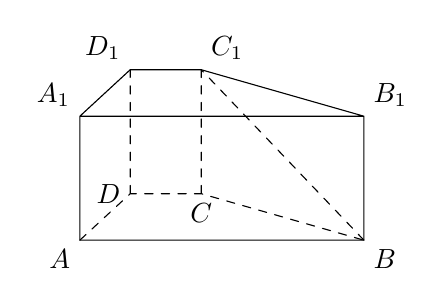
\begin{tikzpicture}[line cap=round,line join=round,x=0.82cm,y=0.82cm]
  \coordinate (A) at (0,0);
  \coordinate (B) at (4.4,0);
  \coordinate (D) at (0.78,0.72);
  \coordinate (C) at (1.88,0.72);
  \coordinate (Aone) at (0,1.92);
  \coordinate (Bone) at (4.4,1.92);
  \coordinate (Done) at (0.78,2.64);
  \coordinate (Cone) at (1.88,2.64);

  % Hidden base and rear vertical edges.
  \draw[dashed] (A)--(D)--(C)--(B) (D)--(Done) (C)--(Cone);
  % Visible lower/front and upper prism edges.
  \draw (A)--(B) (A)--(Aone)--(Bone)--(B)
        (Aone)--(Done)--(Cone)--(Bone);
  % The marked space diagonal BC_1 is dashed in the source.
  \draw[dashed] (B)--(Cone);

  \node[below left] at (A) {$A$};
  \node[below right] at (B) {$B$};
  \node[below] at (C) {$C$};
  \node[left] at (D) {$D$};
  \node[above left] at (Aone) {$A_1$};
  \node[above right] at (Bone) {$B_1$};
  \node[above right] at (Cone) {$C_1$};
  \node[above left] at (Done) {$D_1$};
\end{tikzpicture}
\end{center}
\nopagebreak[4]
\Needspace{4\baselineskip}
\textbf{解析}

\Needspace{5\baselineskip}
取 $A=(0,0,0)$、$B=(4,0,0)$、$D=(0,2,0)$。因 $AB\parallel CD$ 且 $DC=1$，可取 $C=(1,2,0)$；柱高为 $2$，故 $C_1=(1,2,2)$。于是

\nopagebreak[4]
\[
\overrightarrow{BC_1}=(-3,2,2),\qquad \overrightarrow{DC}=(1,0,0)\mbox{。}
\]

\Needspace{5\baselineskip}
两直线夹角取锐角，故其余弦为 $\frac{|\overrightarrow{BC_1}\cdot\overrightarrow{DC}|}{|BC_1||DC|}=\frac3{\sqrt{17}}$，所求角为

\nopagebreak[4]
\[
\arccos\frac3{\sqrt{17}}\mbox{。}
\]

\gkanswer{答案：$\arccos\frac3{\sqrt{17}}$}

\end{answer}
\begin{answer}
\gksolhead{18}{}

\textbf{题目}：

证明：在复数范围内，方程 $|z|^2+(1-i)\overline z-(1+i)z=\dfrac{5-5i}{2+i}$（$i$ 为虚数单位）无解。

\Needspace{4\baselineskip}
\textbf{解析}

\Needspace{5\baselineskip}
写 $z=x+yi$。右端有理化为

\nopagebreak[4]
\[
\frac{5-5i}{2+i}=1-3i\mbox{。}
\]

\Needspace{5\baselineskip}
将左端按实部、虚部分开，可得实部 $x^2+y^2$，虚部 $-2(x+y)$。若等式成立，则

\nopagebreak[4]
\[
x^2+y^2=1,\qquad x+y=\frac32\mbox{。}
\]

但由柯西不等式，$x+y\le\sqrt{2(x^2+y^2)}=\sqrt2<\frac32$，矛盾，故方程无解。

\gkanswer{答案：无解}

\end{answer}
\begin{answer}
\gksolhead{19}{}

\textbf{题目}：

如图，点 $A$、$B$ 分别是椭圆 $\dfrac{x^2}{36}+\dfrac{y^2}{20}=1$ 长轴的左、右端点，点 $F$ 是椭圆的右焦点，点 $P$ 在椭圆上，且位于 $x$ 轴上方，$PA\perp PF$。

（1） 求点 $P$ 的坐标；

（2） 设 $M$ 是椭圆长轴 $AB$ 上的一点，$M$ 到直线 $AP$ 的距离等于 $|MB|$，求椭圆上的点到点 $M$ 的距离 $d$ 的最小值。
\nopagebreak[4]
\begin{center}% Candidate source: src-22a421a422f050bc84accae7bf41feb6903c62df04bd83f34d8267d28f49ee2e
% Source PDF SHA-256: 092e8e90dc1430ab2fa8b8ce79e072e317559e6bef29f1cb7461e9423925ec31
% PDF page 1 (printed page 262), question 19.
% Redraw follows visible relations; point placement is schematic, not a scale claim.
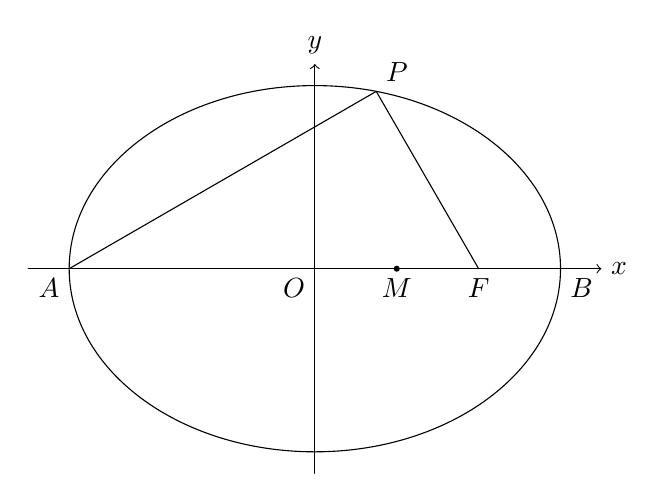
\begin{tikzpicture}[line cap=round,line join=round,x=0.52cm,y=0.52cm]
  \coordinate (A) at (-6,0);
  \coordinate (B) at (6,0);
  \coordinate (F) at (4,0);
  \coordinate (M) at (2,0);
  \coordinate (P) at (1.5,{5*sqrt(3)/2});

  % Ellipse and coordinate axes.
  \draw (0,0) ellipse [x radius=6,y radius={sqrt(20)}];
  \draw[->] (-7,0)--(7,0) node[right] {$x$};
  \draw[->] (0,-5)--(0,5) node[above] {$y$};

  % Chords shown in the source figure.
  \draw (A)--(P)--(F);
  \fill (M) circle (1.1pt);

  \node[below left] at (A) {$A$};
  \node[below right] at (B) {$B$};
  \node[below left] at (0,0) {$O$};
  \node[below] at (M) {$M$};
  \node[below] at (F) {$F$};
  \node[above right] at (P) {$P$};
\end{tikzpicture}
\end{center}
\nopagebreak[4]
\Needspace{4\baselineskip}
\textbf{解析}

\gksubpart{（1）求点 $P$}

\Needspace{5\baselineskip}
椭圆的焦点为 $F=(4,0)$，左端点为 $A=(-6,0)$。由 $PA\perp PF$，

\nopagebreak[4]
\[
(x+6)(x-4)+y^2=0\mbox{。}
\]

结合 $\frac{x^2}{36}+\frac{y^2}{20}=1$，解得 $x=-6$ 或 $x=\frac32$。$x=-6$ 对应端点 $A$，不构成题设中的垂直线段；取椭圆上方的另一点，得 $y=\frac{5\sqrt3}{2}$，所以 $P=(\frac32,\frac{5\sqrt3}{2})$。

\gksubpart{（2）求距离最小值}

设 $M=(m,0)$。由 $A=(-6,0)$、$P=(\frac32,\frac{5\sqrt3}{2})$，有 $|AP|=5\sqrt3$。点 $M$ 到直线 $AP$ 的距离为 $\frac{m+6}{2}$，而 $|MB|=6-m$。条件给出 $\frac{m+6}{2}=6-m$，所以 $m=2$，即 $M=(2,0)$。

\Needspace{5\baselineskip}
椭圆上点到 $M$ 的距离平方为

\nopagebreak[4]
\[
d^2=(x-2)^2+y^2=\frac49x^2-4x+24\mbox{。}
\]

该二次式在 $x=\frac92$ 时取最小值 $15$，且该横坐标对应椭圆上的点，故 $d_{\min}=\sqrt{15}$。

\gkanswer{答案（1）：$P=(\frac32,\frac{5\sqrt3}{2})$}

\gkanswer{答案（2）：$d_{\min}=\sqrt{15}$}

\end{answer}
\begin{answer}
\gksolhead{20}{}

\textbf{题目}：

假设某市 $2004$ 年新建住房面积 $400$ 万平方米，其中有 $250$ 万平方米是中低价房。预计在今后的若干年内，该市每年新建住房面积平均比上一年增长 $8\%$。另外，每年新建住房中，中低价房的面积均比上一年增加 $50$ 万平方米。那么，到哪一年底，

（1） 该市历年所建中低价层的累计面积（以 $2004$ 年为累计的第一年）将首次不少于 $4750$ 万平方米？

（2） 当年建造的中低价房的面积占该年建造住房面积的比例首次大于 $85\%$？

\begin{gktip}
原件第（1）问印作“中低价层”，与本题前文及第（2）问“中低价房”不一致；此处照录原字样，未擅自改写。
\end{gktip}

\Needspace{4\baselineskip}
\textbf{解析}

\gksubpart{（1）累计面积}

\Needspace{5\baselineskip}
按题目前文和第（2）问所用“中低价房”的解释，第 $n$ 年（以 2004 年为第 1 年）新建中低价房面积为 $250+50(n-1)$ 万平方米，前 $n$ 年累计为

\nopagebreak[4]
\[
\sum_{j=1}^{n}\bigl(250+50(j-1)\bigr)=25n(n+9)\mbox{。}
\]

当 $n=9$ 时累计为 $4050$ 万平方米；当 $n=10$ 时为 $4750$ 万平方米，对应 2013 年底。但原题该处印作“中低价层”，不把对“房”的条件性理解冒充原文结论，本问保留 U/PENDING。

\gksubpart{（2）比例首次超过 $85\%$}

\Needspace{5\baselineskip}
第 $n$ 年中低价房与新建住房面积之比为

\nopagebreak[4]
\[
r_n=\frac{200+50n}{400(1.08)^{n-1}}\mbox{。}
\]

相邻比值 $\frac{r_{n+1}}{r_n}=\frac{n+5}{1.08(n+4)}$ 在 $n=1,2,3,4,5$ 时均大于 $1$，所以前六年比例递增。第 5 年约为 $82.69\%$，第 6 年约为 $85.07\%$，首次超过 $85\%$ 是 2009 年底。

\gkanswer{答案（1）：U/PENDING}

\gkanswer{答案（2）：$2009$ 年底}

\end{answer}
\begin{answer}
\gksolhead{21}{}

\textbf{题目}：

\Needspace{5\baselineskip}
对定义域是 $D_f$、$D_g$ 的函数 $y=f(x)$、$y=g(x)$，规定：函数

\nopagebreak[4]
\[
h(x)=
\begin{cases}
f(x)g(x), & \text{\text{当} }x\in D_f\text{ \text{且} }x\in D_g,\\
f(x), & \text{\text{当} }x\in D_f\text{ \text{且} }x\notin D_g,\\
g(x), & \text{\text{当} }x\notin D_f\text{ \text{且} }x\in D_g.
\end{cases}
\]

（1） 若函数 $f(x)=\dfrac{1}{x-1}$，$g(x)=x^2$，写出函数 $h(x)$ 的解析式；

（2） 求问题（1）中函数 $h(x)$ 的值域；

（3） 若 $g(x)=f(x+\alpha)$，其中 $\alpha$ 是常数，且 $\alpha\in[0,\pi]$，请设计一个定义域为 $\mathbb R$ 的函数 $y=f(x)$，及一个 $\alpha$ 的值，使得 $h(x)=\cos4x$，并予以证明。

\Needspace{4\baselineskip}
\textbf{解析}

\gksubpart{（1）写出 $h(x)$}

\Needspace{5\baselineskip}
$D_f=\mathbb R\setminus\{1\}$、$D_g=\mathbb R$。因此

\nopagebreak[4]
\[
h(x)=\begin{cases}
\dfrac{x^2}{x-1},&x\ne1,\\
1,&x=1\mbox{。}
\end{cases}
\]

\gksubpart{（2）求值域}

\Needspace{5\baselineskip}
当 $x\ne1$ 时，设 $y=\frac{x^2}{x-1}$，则关于 $x$ 的方程为 $x^2-yx+y=0$。有实根的条件是判别式 $y^2-4y\ge0$，即 $y\le0$ 或 $y\ge4$。此外 $h(1)=1$，而 $1$ 不在上述值域中，故

\nopagebreak[4]
\[
(-\infty,0]\cup\{1\}\cup[4,+\infty)\mbox{。}
\]

\gksubpart{（3）构造函数}

\Needspace{5\baselineskip}
取 $\alpha=\frac\pi4$，并令

\nopagebreak[4]
\[
f(x)=\sqrt2\cos\left(2x-\frac\pi4\right)\mbox{。}
\]

\Needspace{5\baselineskip}
此时 $D_f=D_g=\mathbb R$，且 $g(x)=f(x+\alpha)=\sqrt2\cos(2x+\frac\pi4)$。利用积化和差，

\nopagebreak[4]
\[
h(x)=f(x)g(x)=\cos\left(-\frac\pi2\right)+\cos4x=\cos4x\text{，}
\]

满足要求。

\gkanswer{答案（1）：$h(x)=\begin{cases}\dfrac{x^2}{x-1},&x\ne1,\\1,&x=1.\end{cases}$}

\gkanswer{答案（2）：$(-\infty,0]\cup\{1\}\cup[4,+\infty)$}

\gkanswer{答案（3）：可取 $\alpha=\frac\pi4$、$f(x)=\sqrt2\cos(2x-\frac\pi4)$}

\end{answer}
\begin{answer}
\gksolhead{22}{}

\textbf{题目}：

在直角坐标平面中，已知点 $P_1(1,2)$，$P_2(2,2^2)$，$P_3(3,2^3)$，$\cdots$，$P_n(n,2^n)$，其中 $n$ 是正整数，对平面上任一点 $A_0$，记 $A_1$ 为 $A_0$ 关于点 $P_1$ 的对称点，$A_2$ 为 $A_1$ 关于点 $P_2$ 的对称点，$\cdots$，$A_n$ 为 $A_{n-1}$ 关于点 $P_n$ 的对称点。

（1） 求向量 $\overrightarrow{A_0A_2}$ 的坐标；

（2） 当点 $A_0$ 在曲线 $C$ 上移动时，点 $A_2$ 的轨迹是函数 $y=f(x)$ 的图象，其中 $f(x)$ 是以 $3$ 为周期的周期函数，且当 $x\in(0,3]$ 时，$f(x)=\lg x$。求以曲线 $C$ 为图象的函数在 $(1,4]$ 上的解析式；

（3） 对任意偶数 $n$，用 $n$ 表示向量 $\overrightarrow{A_0A_n}$ 的坐标。

\Needspace{4\baselineskip}
\textbf{解析}

\gksubpart{（1）求 $\overrightarrow{A_0A_2}$}

\Needspace{5\baselineskip}
连续作两次中心对称，得 $A_2=A_0-2P_1+2P_2$。所以

\nopagebreak[4]
\[
\overrightarrow{A_0A_2}=2(P_2-P_1)=(2,4)\mbox{。}
\]

\gksubpart{（2）求曲线 $C$ 的函数解析式}

\Needspace{5\baselineskip}
若 $A_0=(x,y)$，则 $A_2=(x+2,y+4)$。令 $X=x+2$，则 $y=f(X)-4$。当 $x\in(1,4]$ 时，$X\in(3,6]$；利用 $f$ 的周期为 $3$ 及其在 $(0,3]$ 上等于 $\lg X$，得

\nopagebreak[4]
\[
y=\lg(x-1)-4,\qquad x\in(1,4]\mbox{。}
\]

\gksubpart{（3）求偶数 $n$ 时的向量}

\Needspace{5\baselineskip}
每次中心对称的递推为 $A_k=2P_k-A_{k-1}$。展开递推，偶数 $n$ 时 $A_0$ 的系数为 $1$，于是

\nopagebreak[4]
\[
\overrightarrow{A_0A_n}=2\sum_{j=1}^{n}(-1)^j(j,2^j)\mbox{。}
\]

\Needspace{5\baselineskip}
将正负项两两配对，第一坐标为 $2[(-1+2)+\cdots+(-(n-1)+n)]=n$；第二坐标为 $2\sum_{j=1}^n(-2)^j=\frac{4(2^n-1)}3$。因此

\nopagebreak[4]
\[
\overrightarrow{A_0A_n}=\left(n,\frac{4(2^n-1)}3\right),\qquad n\text{ \text{为正偶数}}\mbox{。}
\]

\gkanswer{答案（1）：$\overrightarrow{A_0A_2}=(2,4)$}

\gkanswer{答案（2）：$y=\lg(x-1)-4$，$x\in(1,4]$}

\gkanswer{答案（3）：$\overrightarrow{A_0A_n}=\left(n,\frac{4(2^n-1)}3\right)$，$n$ 为正偶数}

\end{answer}